%
% fast.tex
%
% (c) 2019 Prof Dr Andreas Müller, Hochschule Rapperswil
%
\section{Schnelle Algorithmen
\label{section:fast}}
\rhead{Schnelle Algorithmen}
Die Basisfunktion $\psi_{j,k}$ geben die Details eines Signals nahe bei
$t=k2^{-j}$ mit einer Auflösung von der Grössenordnung $2^{-j}$ wieder.
Je grösser $j$, desto feiner die Auflösung.
Da die $\psi_{j,k}$ nur eine Basis von $W_j$ sind, werden ausserdem die
Basisfunktion $\varphi_{j,k}$ in mindestens einem der Vektorräume
$V_j$ gebraucht.
Ein praktisch nützlicher Analyse-Algorithmus muss die Koeffizienten
\[
\begin{aligned}
a_{j,k}
&=
\langle f, \varphi_{j,k}\rangle
=
\langle f, D_{2^{-j}}T_k\varphi \rangle
&&&&\text{Mittelwerte}
\\
b_{j,k}
&=
\langle f, \psi_{j,k}\rangle
=
\langle f, D_{2^{-j}}T_k\psi \rangle
&&&&\text{Detail}
\end{aligned}
\]
für jedes beliebige Signal $f$ auf effiziente Art berechnen können.
Dabei wird verwendet, dass die Funktionen  $\varphi_{j,k}$ eine
orthonormierte Basis von $V_j$ sind und die $\psi_{j,k}$ eine
orthonormierte Basis von $W_j$.

\begin{figure}
\centering
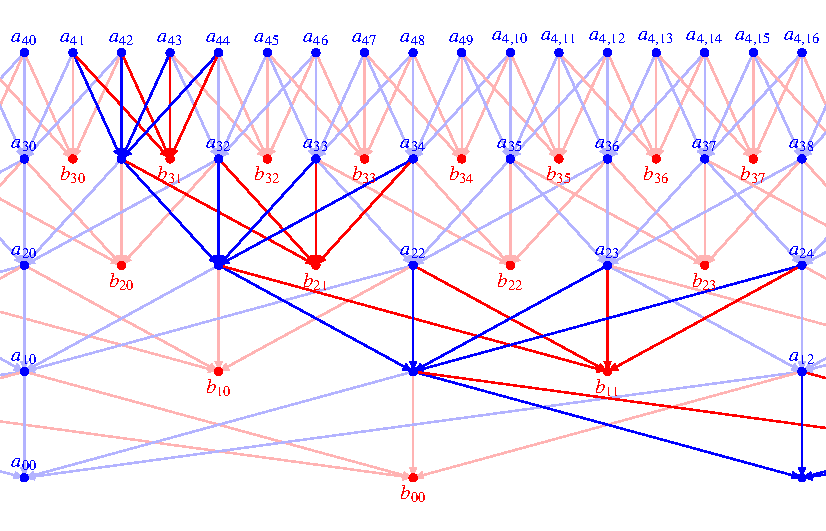
\includegraphics{chapters/7-algo/images/fastalgo.pdf}
\caption{Datenfluss für die Analyse mit vier von $0$ verschiedenen
Koeffizienten $\color{blue}\bar{h}_{-1},\dots,\bar{h}_2$ und
$\color{red}\bar{g}_{-1},\dots,\bar{g}_2$.
Ausgangsdaten für die Analyse sind die Samples $\color{blue}a_{4k}$
in der ersten Zeile.
Durch Anwendung der $\color{blue}h$-Koeffizienten (blaue Linien) können daraus
die Mittelwerte mit gröberer Auflösung $\color{blue}a_{3k}$ gewonnen werden.
Ebenso können durch Anwendung der $\color{red}g$-Koeffizienten (rote Linien)
die Detail-Koeffizienten $\color{red}b_{3k}$ gefunden werden.
Dies wird für jede weitere Detail-Ebene $j$ wiederholt: aus den Koeffizienten
$\color{blue}a_{jk}$ werden mit den $\color{blue}h$-Koeffizienten die
$\color{blue}a_{j+1,k}$ und mit den $\color{red}g$-Koeffizienten die
$\color{red}b_{j+1,k}$ bestimmt.
\label{algo:image:fastalgo}}
\end{figure}

Ein Schlüsselelement einer Multiskalen-Analyse ist die Skalierungsrelation
\begin{align}
\varphi(t) &= \sqrt{2} \sum_{l\in\mathbb Z} h_l \varphi(2t-l)
\notag
\intertext{oder mit den Operatoren $D$ und $T$ geschrieben:}
\varphi    &= \sum_{l\in\mathbb Z} h_l D_{\frac12}T_l\varphi.
\label{algo:formel:phiscale}
\end{align}
Da die Skalierung $D_{\frac12}$ jeden der Vektorräume $V_j$ isometrisch
auf $V_{j+1}$ abbildet, wird daraus eine Skalierungsrelation für alle
Basisfunktionen $\varphi_{j,k}$, die durch Anwendung des Operators
$D_{2^{-j}}T_k$ auf \eqref{algo:formel:phiscale} gefunden werden kann:
\begin{equation}
\varphi_{j,k}
=
D_{2^{-j}}T_k\varphi
=
\sum_{l\in\mathbb Z} h_l D_{2^{-j}} T_k D_{\frac12}T_l \varphi
=
\sum_{l\in\mathbb Z} h_l D_{2^{-j}} D_{\frac12}T_{2k}T_l \varphi
=
\sum_{l\in\mathbb Z} h_l D_{2^{-j-1}} T_{l+2k} \varphi
=
\sum_{l\in\mathbb Z} h_l \varphi_{j+1,l+2k}.
\label{fast:phirelation}
\end{equation}
Im zweitletzten Schritt haben wir die Vertauschungsrelation
$D_{\frac12}T_{2k}=T_{\frac12\cdot2k}D_{\frac12}=T_kD_{\frac12}$
für 
$D_{\frac12}$ und $T_k$ verwendet.
Ausserdem folgt aus der Tatsache, dass $W_j\subset V_{j+1}$ ist,
dass die Basisfunktionen $\psi_{j,k}$ der Orthonormalbasis von $W_j$
Linearkombinationen der Funktionen $\varphi_{j+1,l}$ sein müssen,
die wir als Relation
\[
\psi(t) = \sqrt{2}\sum_{l\in\mathbb Z} g_l \varphi(2t-l),
\]
für das Mutterwavelet schreiben.
Wieder mit Hilfe der Skalierungs-Isometrien $D_{2^{-j}}$ und den
Translationen $T_k$  folgt die entsprechende Relation
\begin{equation}
\psi_{j,k}
=
\sum_{l\in\mathbb Z} g_l D_{2^{-j-1}}T_{l+2k}\varphi
=
\sum_{l\in\mathbb Z} g_l \varphi_{j+1,l+2k}
\label{fast:psirelation}
\end{equation}
für die skalierten und verschobenen Wavelets.

Wendet man die Relationen \eqref{fast:phirelation} und \eqref{fast:psirelation}
auf das Signal $f$ an, indem man das Skalarprodukt mit $f$ bildet,
findet man die Beziehungen
\begin{align}
a_{j,k}
=
\langle f,\varphi_{j,k} \rangle
&=
\sum_{l\in\mathbb Z} \bar{h}_l \langle f,\varphi_{j+1,l+2k}\rangle
=
\sum_{l\in\mathbb Z} \bar{h}_l a_{j+1,l+2k}
\label{fast:akoefgleichung}
\\
b_{j,k}
=
\langle f,\psi_{j,k} \rangle
&=
\sum_{l\in\mathbb Z} \bar{g}_l \langle f,\varphi_{j+1,l+2k}\rangle
=
\sum_{l\in\mathbb Z} \bar{g}_l a_{j+1,l+2k}
\label{fast:bkoefgleichung}
\end{align}
für die Koeffizienten $b_{j,k}$ und $a_{j,k}$.
Die Formeln drücken die Wavelet-Koeffizienten für die Auflösung $j$ durch
die Wavelet-Koeffizienten für die Auflösung $j+1$ aus.
Sobald die Koeffizienten $a_{N,k}$ bekannt sind, können alle Koeffizienten
$a_{j,k}$ mit $j<N$, berechnet werden.

Bleibt die Frage zu klären, woher denn die Koeffizienten $a_{N,k}$ in einer
praktischen Anwendung der Wavelet-Transformation kommen.
Für grosses $j$ ist die Funktion $\varphi_{j,k}$ in der Nähe von $2^{-j}k$
konzentriert.
Ändert das Signal $f$ in einer Umgebung von $2^{-j}k$ nur wenig, kann man
\begin{equation*}
a_{j,k}
=
\langle f,\varphi_{j,k}\rangle
=
\int_{-\infty}^\infty f(t)\, \varphi_{j,k}(t)\,dt
\simeq
f(2^{-j}k)
\int_{-\infty}^\infty \varphi_{j,k}(t)\,dt
\end{equation*}
approximieren.
Bis auf einen möglichen skalaren Faktor gegeben durch das Integral, sind
die Koeffizienten $a_{j,k}$ für genügend grosses $j$ also durch
Sample-Werte $f(2^{-j}k)$ ausreichend genau approximiert.

\begin{beispiel}
Die Skalierungsrelation des Haar-Wavelets hat die Koeffizienten
$h_0=h_1=1$, $g_0=1$ und $g_1=-1$.
Die Berechnung der Koeffizienten gemäss \eqref{fast:akoefgleichung}
und \eqref{fast:bkoefgleichung} führt auf das folgende Berechnungsschema:
\[
\xymatrix{
\dots
	&a_{j,-2} \ar[d] \ar[dr]
		&a_{j,-1} \ar@[red][d]^{\color{red}\cdot (-1)} \ar[dl]
			&a_{j,0} \ar[d] \ar[dr]
				&a_{j,1} \ar@[red][d]^{\color{red}\cdot (-1)} \ar[dl]
					&a_{j,2} \ar[d] \ar[dr]
						&a_{j,3} \ar@[red][d]^{\color{red}\cdot (-1)} \ar[dl]
							&\dots
\\
\dots
	&a_{j-1,-1} \ar@[red][d]^{\color{red}\cdot(-1)}
		&b_{j-1,-1}
			&a_{j-1,0}\ar[d] \ar[drr]
				&b_{j-1,0}
					&a_{j-1,1} \ar@[red][d]^{\color{red}\cdot (-1)} \ar[dll]
						&b_{j-1,1}
							&\dots
\\
\dots &b_{j-2,-1} 
		&
			&a_{j-2,0} \ar[d] \ar[drrrr]
				&
					&b_{j-2,0}
						&
							&\dots \ar[dllll]
\\
\dots &
		&
			&a_{j-3,0}
				&
					&
						&
							&\dots
}
\]
Wo immer zwei Pfeile zusammenkommen, müssen die Terme, von denen die
Pfeile ausgehen, summiert werden.
Rote Pfeile multiplizieren die Ausgangsterme zusätzlich mit $-1$.
\end{beispiel}




